\documentclass{beamer}
\usetheme{metropolis}
\usepackage{pgfpages}
\usepackage{listings}
\usepackage{csquotes}
\usepackage{hyperref}

\ifdefined\NOTES
  \setbeameroption{show only notes}
\fi

\title{Agile Development}
\subtitle{Tools for development}
\author{Kevin Wang \and Aidan Wolk}
\year=2020\relax
\month=01\relax
\day=11\relax
\date{\today}
\institute{DevX}
\logo{
\includegraphics[height=0.5cm]{assets/devxlogo.png}}

\begin{document}

\maketitle

\section{Introduction}

\subsection{Who are we}

\begin{frame}{whoami}
  \begin{columns}
    \begin{column}{0.48\textwidth}
      \textbf{\Large Kevin Wang}

      \begin{description}
        \item[LA Hacks] Tech Director Emeritus
        \item[DevX] Tech Advisor
      \end{description}

      \texttt{\tiny github: @xorkevin}
    \end{column}
    \begin{column}{0.48\textwidth}
      \textbf{\Large Aidan Wolk}

      \begin{description}
        \item[Broomie] Engineering Manager
        \item[DevX] Tech Advisor
      \end{description}

      \texttt{\tiny github: @awolk}
    \end{column}
  \end{columns}
\end{frame}
\note[itemize]{
  \item we are not experts
  \item but we are passionate about developer experience
  \item and want to share our perspectives from our experiences building,
    deploying, and maintaining applications
  \item as your tech advisors, come to us with questions, we are happy to help
}

\subsection{Motivation for this talk}

\begin{frame}{Why is the dev process important?}
  \begin{displayquote}[Anonymous][.]
    A good craftsman never blames his tools
  \end{displayquote}

  A corollary:

  \begin{displayquote}[][.]
    A good craftsman should know his tools
  \end{displayquote}
\end{frame}
\note[itemize]{
  \item an old adage states that a good craftsman should never blame his tools
  \item therefore, a good craftsman should know his tools
  \item working on a tech project is more than just knowing a technology or a
    framework
  \item it involves knowing how to integrate your work with the ecosystem
    around it
  \item thus, you need to know your tools, their capabilities, and their
    limitations
}

\begin{frame}{Brief Overview}
  \begin{itemize}
    \item Version Control
      \begin{itemize}
        \item Git
        \item best practices
      \end{itemize}
    \item Containerization
      \begin{itemize}
        \item Docker
        \item How to begin using it
      \end{itemize}
  \end{itemize}
\end{frame}
\note[itemize]{
  \item you have probably heard of these tools before
  \item if not, do not worry, that is what this talk is for
  \item we want to focus on best practices for using these tools and how you
    can incorporate them into your project
}

\section{Version Control}

\subsection{What is it}

\begin{frame}{Version Control}
  \begin{itemize}
    \item history tracking for files
    \item no more saving multiple copies manually
    \item changes can be committed and tracked by the VCS
    \item modern VCS's can easily merge changesets (like you will need for your
      projects)
  \end{itemize}
\end{frame}
\note[itemize]{
  \item every project should be using version control
  \item aside from making collaboration easier, it allows you to view the
    history of your own changes
  \item helpful for identifying which changes introduced bugs
}

\begin{frame}{How did we get here?}
  \begin{description}
    \item[SCCS] Bell Labs, 1972, early software VCS
    \item[RCS] Purdue, 1982, delta storage
    \item[CVS] University Amsterdam, 1986, multi-user
    \item[SVN] CollabNet, 2000, spiritual successor of CVS
    \item[Git] Linus Torvalds, 2005, distributed VCS
  \end{description}
\end{frame}
\note[itemize]{
  \item Source code control system, one of the first software VCS, major
    upgrade over punch cards, kept track of single files, single user
  \item Revision control sytem, tracked diffs between versions
  \item Concurrent versions system, developed for MINIX development, can work
    across the network, centralized development
  \item Subversion, spiritual successor of CVS
  \item Git, developed to maintain Linux development after Bitkeeper license
    changes
}

\subsection{Git}

\begin{frame}{Why Git?}
  \begin{center}
    
\includegraphics[height=0.75cm]{assets/gitlogo.png}
  \end{center}
  \begin{itemize}
    \item Distributed version control system
      \begin{itemize}
        \item multiple independent branches across computers
        \item No branch is inherently “more important” than the other
      \end{itemize}
    \item High industry adoption
    \item Most popular source code repository hosting services e.g. GitHub,
      GitLab use Git
    \item \href{https://www.youtube.com/watch?v=4XpnKHJAok8}{Youtube - Tech
      Talk: Linus Torvalds on git}
  \end{itemize}
\end{frame}
\note[itemize]{
  \item we highly encourage you to use Git
  \item Git makes merging easy
  \item merging in non-distributed VCS is hard
  \item anyone who has tried working with SVN or CVS knows this
  \item Mercurial is also a DVCS, however usage is small compared to Git
}

\section{Git}

\subsection{Conceptual overview}

\begin{frame}{Distributed VCS}
  \begin{center}
    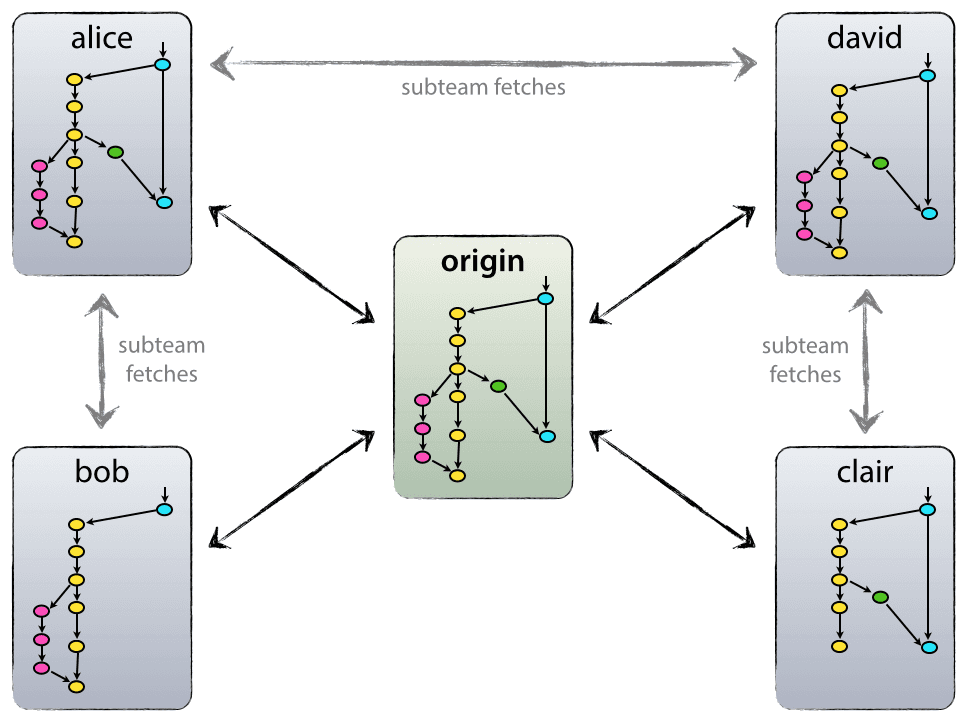
\includegraphics[width=\textwidth]{assets/gitdistributed.png}
  \end{center}
\end{frame}
\note[itemize]{
  \item understanding Git conceptually is important before you begin working
    with its commands
  \item a Git repository is the collection of changes for a set of files
  \item because Git is a DVCS, it has no concept of a central repo that
    everyone must checkin code to
  \item everyone has their own copy of the repository that they can clone to
    work off of
  \item in practice, one of these copies of the repo will be designated the
    central source of truth copy, typically called origin and hosted at an
    easily accessible location like GitHub or GitLab, and it will serve as the
    method to send changes between team members
}

\begin{frame}{Commit graph}
  \begin{center}
    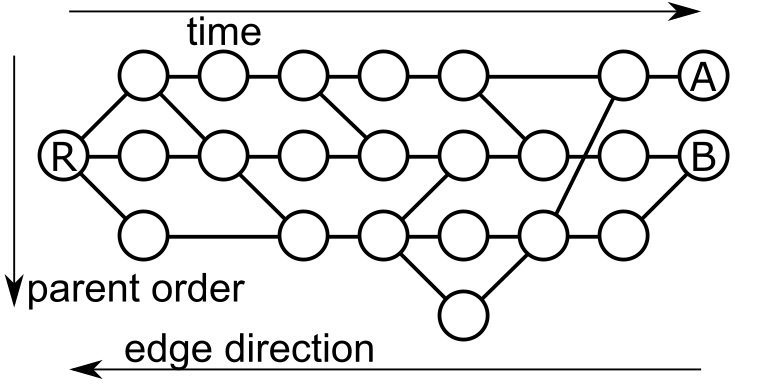
\includegraphics[width=\textwidth]{assets/gitgraph.png}
  \end{center}
\end{frame}
\note[itemize]{
  \item changes in Git are organized in the form of commits
  \item a commit is conceptually a set of changed lines from an earlier commit
  \item these commits form a directed acyclic graph which encompass all the
    changes which have been checked in to a repository
}

\begin{frame}{Workflow}
  \begin{center}
    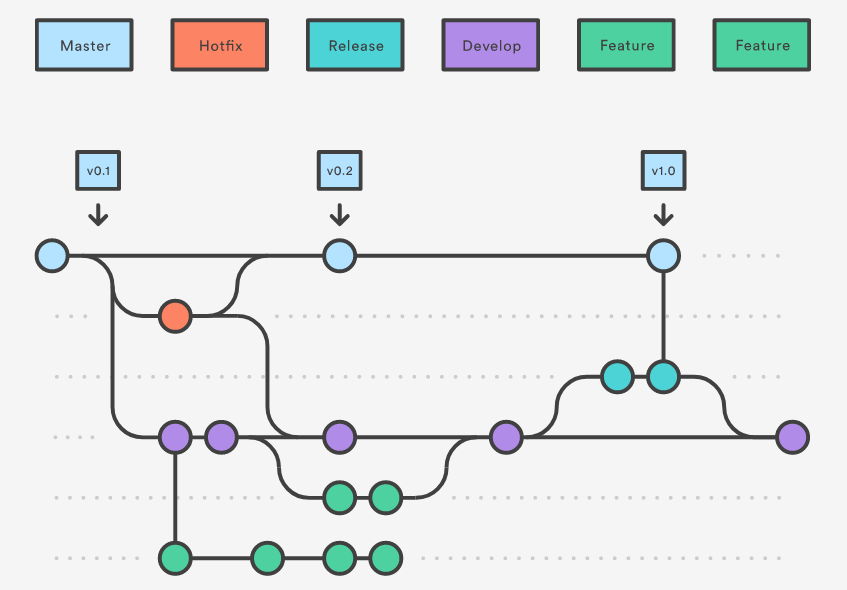
\includegraphics[width=\textwidth]{assets/gitworkflow.png}
  \end{center}
\end{frame}
\note[itemize]{
  \item Git is quite flexible and supports many workflows
  \item some teams prefer more trunk based development, where everyone commits
    to the same upstream origin branch, typically called master
    \begin{itemize}
      \item usually for small projects
    \end{itemize}
  \item larger projects need a more scalable way to manage changes
  \item typically will have a production, development, and feature branches
  \item team members will work on their own features and merge them into the
    development branch when they are finished
  \item use a flow that works best for you
}

\begin{frame}{Git}
  \Huge Demo
\end{frame}

\subsection{Best practices}

\begin{frame}{.gitignore}
  \begin{itemize}
    \item Only source code should be checked in
      \begin{itemize}
        \item Do \textbf{not} commit build artifacts to your repo
      \end{itemize}
    \item When X is reproducible from Y, X does not need to be checked in 99\%
      of the time.
      \begin{itemize}
        \item e.g. \texttt{node\_modules/} is reproducible from
          \texttt{package-lock.json}
      \end{itemize}
  \end{itemize}
\end{frame}
\note[itemize]{
  \item Too often I see \texttt{.DS\_Store} or \texttt{\_\_MACOSX} committed
  \item those files should be ignored in your personal global
    \texttt{.gitignore}
}

\begin{frame}{More helpful Git}
  \begin{itemize}
    \item Commit \textbf{early} and \textbf{often}. Commits should be thought
      of as an atomic unit of work.
    \item Rebase with care. Feel free to rebase your own work that you have
      locally. But, do \textbf{not} rebase public history. Doing so will
      rewrite history for others, and Git will not be able to help you merge
      changes.
    \item \texttt{git bisect}. Binary search your history for a bug introducing
      commit.
    \item \texttt{git diff}, \texttt{git apply}, \texttt{git cherry-pick}.
      These commands can help you with complex or out-of-tree merges if you
      need it.
    \item \texttt{git blame}. Find which commit added a particular line.
  \end{itemize}
\end{frame}
\note[itemize]{
  \item Git provides many helpful commands to manage your work, and work with
    others.
  \item One can better leverage these tools by adhering to good conventions.
}

\end{document}
